\chapter{Case study}\label{chap:case}
Dynamic languages with a garbage collector have the advantage of letting the programmer use the exploratory style of programming, where he doesn't have to worry about memory management or other low level considerations. [][] Doesn't have to design a complex type hierarchy or any similar scaffolding. He can just jump in and start implementing an idea. This is excellent for prototyping.

But when it comes to performance and robustness this approach shows its downsides very quickly. The safety of static types combined with a good development environment catches a lot of bugs and inconsistencies before runtime. Garbage collector mechanisms vary in implementation, each showing a different performance characteristic. In this chapter I will describe the implementation of a clone of Pac-Man in Dual and performance issues that I've encountered. These are very much related to the JavaScript environment, notably the event loop and the garbage collector, which has different implementations across browsers. The latter did shows a significant difference when comparing different web browsers.

Implementation of a non-trivial application allows to test the language design and quickly establish which features are the most useful in practice.
I found that I could do away with a lot of the more complex ones %% performance gain, net win

\section{The game}
\begin{figure}[h!]
\centering
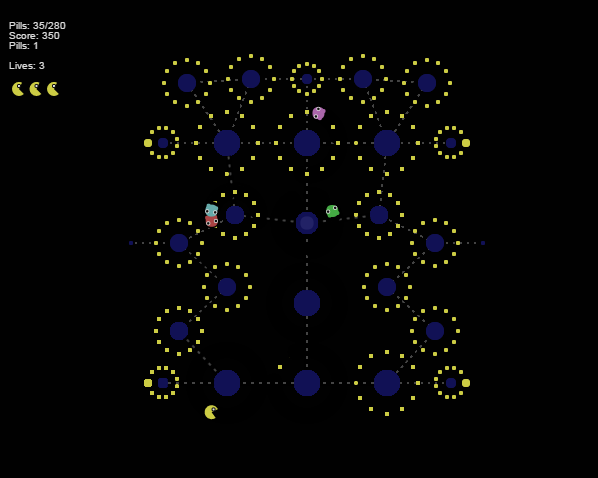
\includegraphics[width=0.9\textwidth]{pacman}
\caption{A screenshot from the game}
\label{fig:pacman}
\end{figure}

% put a firefox version as a separate example

\subsection{Main loop}

\section{Performance}


pacman

vs Links
vs JS
vs Unreal Engine
    BLUI
    Coherent
        web platform for UIs everywhere

early user feedback

event loop
js event model
fight with garbage collector
game loop
requestAnimationFrame

Ten rozdział zawiera opis wyników uzyskanych w~ramach pracy. Jeśli praca miała
cel badawczy należy skupić się na opisie przeprowadzonych eksperymentów oraz
prezentacji i~analizie uzyskanych wyników. Jeśli praca nie miała na celu
uzyskania nowatorskich wyników, należy skupić się na opisie architektury
stworzonej aplikacji. W~obu przypadkach podstawowym celem tego rozdziału jest
realizacja celów postawionych w~rozdziale \ref{sec:cele_pracy}. Rozdział ten ma
bezspornie pokazywać, że cele pracy zostały zrealizowane
